\documentclass{beamer}

%
% Common preamble for all three parts.
%

\usepackage[brazil,english]{babel}
\usepackage[utf8]{inputenc}
\usepackage{amsmath}
\usepackage{color}
\usepackage{minted}
\usepackage{hyperref}
\usepackage{multicol}
\usepackage{tabularx}
\usepackage{tikz}

% only inline todonotes work
\usepackage{xkeyval}
\usepackage[textsize=small]{todonotes}
\presetkeys{todonotes}{inline}{}

\usetikzlibrary{shapes,arrows,positioning,shadows}

% no nav buttons
\usenavigationsymbolstemplate{}

\newcommand{\bftt}[1]{\textbf{\texttt{#1}}}
\newcommand{\comment}[1]{{\color[HTML]{008080}\textit{\textbf{\texttt{#1}}}}}
\newcommand{\cmd}[1]{{\color[HTML]{008000}\bftt{#1}}}
\newcommand{\bs}{\char`\\}
\newcommand{\cmdbs}[1]{\cmd{\bs#1}}
\newcommand{\lcb}{\char '173}
\newcommand{\rcb}{\char '175}
\newcommand{\cmdbegin}[1]{\cmdbs{begin\lcb}\bftt{#1}\cmd{\rcb}}
\newcommand{\cmdend}[1]{\cmdbs{end\lcb}\bftt{#1}\cmd{\rcb}}

\newcommand{\wllogo}{\textbf{write\textrm{\LaTeX}}}

% this is where the example source files are loaded from
% do not include a trailing slash
%\newcommand{\fileuri}{https://raw.github.com/jdleesmiller/latex-course/master/en}
\newcommand{\fileuri}{https://raw.githubusercontent.com/jmetzz/latex-course/master/pt-br}

\newcommand{\wlserver}{https://www.writelatex.com}
\newcommand{\wlnewdoc}[1]{\wlserver/docs?snip\_uri=\fileuri/#1\&splash=none}

\def\tikzname{Ti\emph{k}Z}

% from http://tex.stackexchange.com/questions/5226/keyboard-font-for-latex
\newcommand*\keystroke[1]{%
  \tikz[baseline=(key.base)]
    \node[%
      draw,
      fill=white,
      drop shadow={shadow xshift=0.25ex,shadow yshift=-0.25ex,fill=black,opacity=0.75},
      rectangle,
      rounded corners=2pt,
      inner sep=1pt,
      line width=0.5pt,
      font=\scriptsize\sffamily
    ](key) {#1\strut}
  ;
}
\newcommand{\keystrokebftt}[1]{\keystroke{\bftt{#1}}}

% stolen from minted.dtx
\newenvironment{exampletwoup}
  {\VerbatimEnvironment
   \begin{VerbatimOut}{example.out}}
  {\end{VerbatimOut}
   \setlength{\parindent}{0pt}
   \fbox{\begin{tabular}{l|l}
   \begin{minipage}{0.55\linewidth}
     \inputminted[fontsize=\small,resetmargins]{latex}{example.out}
   \end{minipage} &
   \begin{minipage}{0.35\linewidth}
     \input{example.out}
   \end{minipage}
   \end{tabular}}}

\newenvironment{exampletwouptiny}
  {\VerbatimEnvironment
   \begin{VerbatimOut}{example.out}}
  {\end{VerbatimOut}
   \setlength{\parindent}{0pt}
   \fbox{\begin{tabular}{l|l}
   \begin{minipage}{0.55\linewidth}
     \inputminted[fontsize=\scriptsize,resetmargins]{latex}{example.out}
   \end{minipage} &
   \begin{minipage}{0.35\linewidth}
     \setlength{\parskip}{6pt plus 1pt minus 1pt}%
     \raggedright\scriptsize\input{example.out}
   \end{minipage}
   \end{tabular}}}

\newenvironment{exampletwouptinynoframe}
  {\VerbatimEnvironment
   \begin{VerbatimOut}{example.out}}
  {\end{VerbatimOut}
   \setlength{\parindent}{0pt}
   \begin{tabular}{l|l}
   \begin{minipage}{0.55\linewidth}
     \inputminted[fontsize=\scriptsize,resetmargins]{latex}{example.out}
   \end{minipage} &
   \begin{minipage}{0.35\linewidth}
     \setlength{\parskip}{6pt plus 1pt minus 1pt}%
     \raggedright\scriptsize\input{example.out}
   \end{minipage}
   \end{tabular}}

\title{Uma Introdução Interativa ao \LaTeX}
\author{Dr John D. Lees-Miller}


\titlegraphic{%

\includegraphics[page=4]{wllogo-series}\\[1em]

\includegraphics[height=24pt]{UoB-logo}
\qquad

\includegraphics[height=24pt]{setsquared_supported}
}





\subtitle{Parte 1: Conceitos Básicos}

\begin{document}

%%%%%%%%%%%%%%%%%%%%%%%%%%%%%%%%%%%%%%%%%%%%%%%%%%%%%%%%%%%%%%%%%%%%%%%%%%%%%%%
%%%%%%%%%%%%%%%%%%%%%%%%%%%%%%%%%%%%%%%%%%%%%%%%%%%%%%%%%%%%%%%%%%%%%%%%%%%%%%%
%%%%%%%%%%%%%%%%%%%%%%%%%%%%%%%%%%%%%%%%%%%%%%%%%%%%%%%%%%%%%%%%%%%%%%%%%%%%%
\begin{frame}
	\titlepage
\end{frame}


\input{credits}

\section{Introdução}
%%%%%%%%%%%%%%%%%%%%%%%%%%%%%%%%%%%%%%%%%%%%%%%%%%%%%%%%%%%%%%%%%%%%%%%%%%%%%%%
%%%%%%%%%%%%%%%%%%%%%%%%%%%%%%%%%%%%%%%%%%%%%%%%%%%%%%%%%%%%%%%%%%%%%%%%%%%%%%%
%%%%%%%%%%%%%%%%%%%%%%%%%%%%%%%%%%%%%%%%%%%%%%%%%%%%%%%%%%%%%%%%%%%%%%%%%%%%%%%
\begin{frame}{Por que \LaTeX{}?}
	\begin{itemize}
		\item Ele faz documentos bonitos e bem formatados
			\begin{itemize}
				\item Especialmente com conteúdo matemático
			\end{itemize}
%
		\item Ele foi criado por cientistas, para cientistas
			\begin{itemize}
				\item Há uma grande e ativa comunidade
			\end{itemize}
%
		\item Ele é poderoso --- e você pode estendê-lo
			\begin{itemize}
				\item Existem pacotes para artigos, apresentações, planilhas eletrônicas,  \ldots
			\end{itemize}
	\end{itemize}
\end{frame}


\begin{frame}{Vantagens ao usar \LaTeX{}?}
	\begin{itemize}\scriptsize
		\item O padrão matemático em \TeX{} gera equações e funções corretamente formatadas. Em Word, o editor de equações está longe de ser ideal.
		\item \TeX{} não tem \textit{bugs} — o Word, como sabemos, está recheado de \textit{bugs}.
		\item \TeX{} é gratuito e livre.
		\item Em \TeX{}, você pode comentar o seu código/texto no mesmo espaço em que seu conteúdo é gerado.
		\item \TeX{} oferece uma linguagem completa. Ou seja: você pode criar funções que efetuam um procedimento para você (muitas dessas funções não podem ser criadas via macros em Word).
		\item Não há vírus de macros em \TeX. Ou seja: maior segurança.
		\item Não há incompatibilidade de versões: se você criou um arquivo \TeX{} em 1995, conseguirá abri-lo perfeitamente hoje.
		\item \LaTeX{} oferece uma maneira independente de lidar com bibliografias. Nada de comprar \textit{EndNote} ou algo parecido: toda a sua biblioteca de referências é mantida em um simples arquivo, ao qual você conecta citações.
		\item Documentos em \TeX{} são pequenos (em bytes).
		\item \LaTeX{} é o padrão científico/acadêmico em diversas áreas do conhecimento — e nos maiores centros acadêmicos do mundo.
		\item \LaTeX{} gera documentos mais aprimorados esteticamente, com menos hifenizações e menos espaçamentos exagerados entre palavras.
		\item Seu \texttt{pdf} é gerado com uma estrutura interna, em que você acessa seções via \textit{links} — isso é feito automaticamente com um pacote específico.
	\end{itemize}
\end{frame}

%%%%%%%%%%%%%%%%%%%%%%%%%%%%%%%%%%%%%%%%%%%%%%%%%%%%%%%%%%%%%%%%%%%%%%%%%%%%%%%
%%%%%%%%%%%%%%%%%%%%%%%%%%%%%%%%%%%%%%%%%%%%%%%%%%%%%%%%%%%%%%%%%%%%%%%%%%%%%%%
%%%%%%%%%%%%%%%%%%%%%%%%%%%%%%%%%%%%%%%%%%%%%%%%%%%%%%%%%%%%%%%%%%%%%%%%%%%%%%%
\begin{frame}[fragile]{Ajuste de atitude}

\begin{itemize}
	\item Use comandos para descrever `o que é', não `como parece'.
	\item Foque no conteúdo.
	\item Deixe que o \LaTeX{} faça o trabalho.
\end{itemize}
\end{frame}

%%%%%%%%%%%%%%%%%%%%%%%%%%%%%%%%%%%%%%%%%%%%%%%%%%%%%%%%%%%%%%%%%%%%%%%%%%%%%%%%
%%%%%%%%%%%%%%%%%%%%%%%%%%%%%%%%%%%%%%%%%%%%%%%%%%%%%%%%%%%%%%%%%%%%%%%%%%%%%%%%
%%%%%%%%%%%%%%%%%%%%%%%%%%%%%%%%%%%%%%%%%%%%%%%%%%%%%%%%%%%%%%%%%%%%%%%%%%%%%%%%
\begin{frame}[fragile]{Como ele funciona?}
\begin{itemize}
\item Você escreve seu documento em \texttt{texto puro} com \cmd{comandos} que descrevem a estrutura e significado do texto.

\item O programa \texttt{latex} processa seu texto e comandos para produzir um documento bem formatado e bonito.
\end{itemize}
\vskip 2ex
\begin{center}
\begin{minted}[frame=single]{latex}
A chuva na Espanha cai \emph{principalmente} 

na plan\'icie.
\end{minted}
\vskip 2ex
\tikz\node[single arrow,fill=gray,font=\ttfamily\bfseries,%
  rotate=270,xshift=-1em]{latex};
\vskip 2ex
\fbox{A chuva na Espanha cai \emph{principalmente} na planície.}
\end{center}
\end{frame}

%%%%%%%%%%%%%%%%%%%%%%%%%%%%%%%%%%%%%%%%%%%%%%%%%%%%%%%%%%%%%%%%%%%%%%%%%%%%%%%
%%%%%%%%%%%%%%%%%%%%%%%%%%%%%%%%%%%%%%%%%%%%%%%%%%%%%%%%%%%%%%%%%%%%%%%%%%%%%%%
%%%%%%%%%%%%%%%%%%%%%%%%%%%%%%%%%%%%%%%%%%%%%%%%%%%%%%%%%%%%%%%%%%%%%%%%%%%%%%%
\begin{frame}[fragile]{Inconveniente}

\begin{itemize}
	\item Por padrão, os acentos não são como em editores de texto :(
	
	Lembrem-se que foi incialmente desenvolvido para Inglês (não há acentos)

	\item Devemos usar caracteres de escape para acentuar palavras: 
	 \keystrokebftt{\bs} seguido do símoblo que representa o acento, 
	 seguido da letra que deve ser acentuada. Exemplo:
\end{itemize}

	\begin{exampletwoup}
			\'a, \~a, \^a, \`a
	\end{exampletwoup}


\end{frame}


%%%%%%%%%%%%%%%%%%%%%%%%%%%%%%%%%%%%%%%%%%%%%%%%%%%%%%%%%%%%%%%%%%%%%%%%%%%%%%%
%%%%%%%%%%%%%%%%%%%%%%%%%%%%%%%%%%%%%%%%%%%%%%%%%%%%%%%%%%%%%%%%%%%%%%%%%%%%%%%
%%%%%%%%%%%%%%%%%%%%%%%%%%%%%%%%%%%%%%%%%%%%%%%%%%%%%%%%%%%%%%%%%%%%%%%%%%%%%%%
\begin{frame}[fragile]{Mais exemplos de comandos e suas respectivas saídas \ldots}
	\begin{exampletwoup}
		\begin{itemize}
			\item Ch\'a
			\item Leite
			\item Biscoito
		\end{itemize}
	\end{exampletwoup}
\vskip 2ex
	\begin{exampletwoup}
		\begin{figure}
			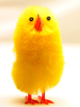
\includegraphics{chick}
		\end{figure}
	\end{exampletwoup}
\vskip 2ex
	\begin{exampletwoup}
		\begin{equation}
			\alpha + \beta + 1
		\end{equation}
	\end{exampletwoup}

	\tiny{Image from \url{http://www.andy-roberts.net/writing/latex/importing_images}}
\end{frame}


%%%%%%%%%%%%%%%%%%%%%%%%%%%%%%%%%%%%%%%%%%%%%%%%%%%%%%%%%%%%%%%%%%%%%%%%%%%%%%%
%%%%%%%%%%%%%%%%%%%%%%%%%%%%%%%%%%%%%%%%%%%%%%%%%%%%%%%%%%%%%%%%%%%%%%%%%%%%%%%
%%%%%%%%%%%%%%%%%%%%%%%%%%%%%%%%%%%%%%%%%%%%%%%%%%%%%%%%%%%%%%%%%%%%%%%%%%%%%%%
\section{Básico}
%%%%%%%%%%%%%%%%%%%%%%%%%%%%%%%%%%%%%%%%%%%%%%%%%%%%%%%%%%%%%%%%%%%%%%%%%%%%%%%
%%%%%%%%%%%%%%%%%%%%%%%%%%%%%%%%%%%%%%%%%%%%%%%%%%%%%%%%%%%%%%%%%%%%%%%%%%%%%%%
%%%%%%%%%%%%%%%%%%%%%%%%%%%%%%%%%%%%%%%%%%%%%%%%%%%%%%%%%%%%%%%%%%%%%%%%%%%%%%%
\subsection{Ferramentas}
\begin{frame}[fragile]{\insertsubsection {} para edição}
	\begin{itemize}
		\item \wllogo{} ... online e colaborativo
		\item TexMaker ... free
		\item \TeX works ... padrão do Mik\TeX
		\item WinShell ... free
		\item TexNicCenter ... free
		\item WinEdt ... pago :(
		\item \ldots
	\end{itemize}
\end{frame}

\begin{frame}[fragile]{\insertsubsection {} para compilação}
	\begin{itemize}
		\item Mik\TeX{} - Windows
		\item \TeX Live ou tetex - *nix
		\item Mac\TeX{} - Mac OS 
		\vskip 3ex
		\item ou use o \wllogo{} para não se incomodar com a instalação da plataforma!
	\end{itemize}
\end{frame}


%%%%%%%%%%%%%%%%%%%%%%%%%%%%%%%%%%%%%%%%%%%%%%%%%%%%%%%%%%%%%%%%%%%%%%%%%%%%%%%
%%%%%%%%%%%%%%%%%%%%%%%%%%%%%%%%%%%%%%%%%%%%%%%%%%%%%%%%%%%%%%%%%%%%%%%%%%%%%%%
%%%%%%%%%%%%%%%%%%%%%%%%%%%%%%%%%%%%%%%%%%%%%%%%%%%%%%%%%%%%%%%%%%%%%%%%%%%%%%%
\subsection{Começando}
\begin{frame}[fragile]{\insertsubsection}
\begin{itemize}
	\item Um documento \LaTeX{} mínimo:
		\inputminted[frame=single]{latex}{basics.tex}
	
	\item Comandos começam com  \emph{backslash} \keystrokebftt{\bs}.
	\item Todo documento comaça com um comando \cmdbs{documentclass}.
	\item O \emph{argumento} dentro das chaves \keystrokebftt{\{} \keystrokebftt{\}} representam que tipo de documento \LaTeX{} estamos criando: um \bftt{article}.
	\item O símbolo de percentual \keystrokebftt{\%} é usado para marcar o início de \emph{comentários} --- o \LaTeX{} vai ignorar o restante da linha.
\end{itemize}
\end{frame}


%%%%%%%%%%%%%%%%%%%%%%%%%%%%%%%%%%%%%%%%%%%%%%%%%%%%%%%%%%%%%%%%%%%%%%%%%%%%%%%
%%%%%%%%%%%%%%%%%%%%%%%%%%%%%%%%%%%%%%%%%%%%%%%%%%%%%%%%%%%%%%%%%%%%%%%%%%%%%%%
%%%%%%%%%%%%%%%%%%%%%%%%%%%%%%%%%%%%%%%%%%%%%%%%%%%%%%%%%%%%%%%%%%%%%%%%%%%%%%%
\begin{frame}[fragile]{\insertsubsection{} com \wllogo}
	\begin{itemize}
		\item write\LaTeX{} é um \textit{website} para escrita de documentos em \LaTeX.
		\item Ele `compila' seu código \LaTeX{} automaticamente para te mostrar o resultado.
			\vskip 2em
			\begin{center}
				\fbox{\href{\wlnewdoc{basics.tex}}{Clique aqui para abrir um exemplo de documento no \wllogo{}}}
				\\[1ex]\scriptsize{}
				Ou v\'a para essa URL: \url{http://bit.ly/WU0bMU}\\
				Para melhores resultados, por favor use \href{http://www.google.com/chrome}{Google Chrome} ou uma vers\~ao recente do \href{http://www.mozilla.org/en-US/firefox/new/}{FireFox}.
			\end{center}
		\vskip 2ex
		\item Conforme passamos pelos próximos \textit{slides}, teste os exemplos os digitando no documento de exemplo no \wllogo.
		\item \textbf{Não agora. Você deve testá-los conforme vamos passando pelos exemplos!}
	\end{itemize}
\end{frame}

%%%%%%%%%%%%%%%%%%%%%%%%%%%%%%%%%%%%%%%%%%%%%%%%%%%%%%%%%%%%%%%%%%%%%%%%%%%%%%%
%%%%%%%%%%%%%%%%%%%%%%%%%%%%%%%%%%%%%%%%%%%%%%%%%%%%%%%%%%%%%%%%%%%%%%%%%%%%%%%
%%%%%%%%%%%%%%%%%%%%%%%%%%%%%%%%%%%%%%%%%%%%%%%%%%%%%%%%%%%%%%%%%%%%%%%%%%%%%%%
\subsection{Compondo o Texto}
\begin{frame}[fragile]{\insertsubsection{}}
	\small
	\begin{itemize}
		\item Digite seu texto entre \cmdbegin{document} e \cmdend{document}.
		\item Para a maior parte, você pode apenas digitar seu texto normalmente.
	\begin{exampletwouptiny}
		Palavras s\~ao separadas por um ou 
		mais espa\c{c}os.
		
		Par\'agrafos s\~ao separados por uma 
		ou mais linhas em branco.
	\end{exampletwouptiny}
	\item Espaços no arquivo fonte são truncados no arquivo de saída.
		\begin{exampletwouptiny}
			A     chuva      na Espanha
			cai principalmente na plan\'icie.
		\end{exampletwouptiny}
	\end{itemize}
\end{frame}

%%%%%%%%%%%%%%%%%%%%%%%%%%%%%%%%%%%%%%%%%%%%%%%%%%%%%%%%%%%%%%%%%%%%%%%%%%%%%%%
%%%%%%%%%%%%%%%%%%%%%%%%%%%%%%%%%%%%%%%%%%%%%%%%%%%%%%%%%%%%%%%%%%%%%%%%%%%%%%%
%%%%%%%%%%%%%%%%%%%%%%%%%%%%%%%%%%%%%%%%%%%%%%%%%%%%%%%%%%%%%%%%%%%%%%%%%%%%%%%
\begin{frame}[fragile]{\insertsubsection{}: Cuidado}
\small
	\begin{itemize}
	\item Aspas são um pouco complicadas: use crase \keystroke{\`{}} à esquerda e apóstrofe \keystroke{\'{}} à direita.
		\begin{exampletwouptiny}
			Aspas simples: `texto'.
	
			Aspas duplas: ``texto''.
		\end{exampletwouptiny}
	
	\item Em \LaTeX{} alguns caracteres comuns são especiais :\\[1ex]
		\begin{tabular}{cl}
			\keystrokebftt{\%} & símbolo percentual              \\
			\keystrokebftt{\#} & cerquilha  \\
			\keystrokebftt{\&} & e-comercial                 \\
			\keystrokebftt{\$} & cifrão               \\
		\end{tabular}
	\item Se você apenas digitá-los, terá um erro como resultado. Se você quer que um desses caracteres apareça na saída, terá que usar um caractere de \emph{escape} como prefixo: a barra invertida \keystrokebftt{$\backslash$}.
		\begin{exampletwoup}
			\$\%\&\#!
		\end{exampletwoup}
	\end{itemize}
\end{frame}

%%%%%%%%%%%%%%%%%%%%%%%%%%%%%%%%%%%%%%%%%%%%%%%%%%%%%%%%%%%%%%%%%%%%%%%%%%%%%%%
%%%%%%%%%%%%%%%%%%%%%%%%%%%%%%%%%%%%%%%%%%%%%%%%%%%%%%%%%%%%%%%%%%%%%%%%%%%%%%%
%%%%%%%%%%%%%%%%%%%%%%%%%%%%%%%%%%%%%%%%%%%%%%%%%%%%%%%%%%%%%%%%%%%%%%%%%%%%%%%
\begin{frame}[fragile]{Tratando Erros}
	\begin{itemize}
		\item O compilador \LaTeX{} pode se confundir quando estiver tentanto 
		compilar o seu documento. Se isso acontecer, ele para e apresenta um erro, 
		o qual você deve corrigir antes que ele possa produzir o arquivo de saída.
		
		\item Por exemplo, se voc\^e digitar erroneamente \cmdbs{emph} como \cmdbs{meph},
		o \LaTeX{} vai parar com o erro ``undefined control sequence'', pois ``meph'' não 
		é um dos comandos conhecidos.
	\end{itemize}
	
	\begin{block}{Dicas em caso de erros}
		\begin{enumerate}
			\item \alert{Don't panic}! Erros acontecem.
			\item Corrija assim que eles aparecerem --- se o que voc\^e acabou de digitar causou um erro, voc\^e pode \textit{debuggar} a partir desse ponto.
			\item Se existem m\'ultiplos erros, comece com o primeiro --- a causa pode estar acima dele :(
		\end{enumerate}
	\end{block}
\end{frame}

%%%%%%%%%%%%%%%%%%%%%%%%%%%%%%%%%%%%%%%%%%%%%%%%%%%%%%%%%%%%%%%%%%%%%%%%%%%%%%%
%%%%%%%%%%%%%%%%%%%%%%%%%%%%%%%%%%%%%%%%%%%%%%%%%%%%%%%%%%%%%%%%%%%%%%%%%%%%%%%
%%%%%%%%%%%%%%%%%%%%%%%%%%%%%%%%%%%%%%%%%%%%%%%%%%%%%%%%%%%%%%%%%%%%%%%%%%%%%%%
\begin{frame}[fragile]{Compondo o Texto - Exerc\'icio 1}

	\begin{block}{Digite isso em \LaTeX:
	\footnote{\url{http://en.wikipedia.org/wiki/Economy_of_the_United_States}}}
		In March 2006, Congress raised that ceiling an additional \$0.79 trillion to
		\$8.97 trillion, which is approximately 68\% of GDP. As of October 4, 2008, the
		``Emergency Economic Stabilization Act of 2008'' raised the current debt ceiling
		to \$11.3 trillion.
	\end{block}
	\vskip 2ex
	\begin{center}
		\fbox{\href{\wlnewdoc{basics-exercise-1.tex}}{%
		Clique no \wllogo{} para abrir esse exerc\'icio}}
	\end{center}
	
	\begin{itemize}
		\item Dica: cuidado com os caracteres com significado especial!
		\item Uma vez que você tenha tentando, 
			\fbox{\href{\wlnewdoc{basics-exercise-1-solution.tex}}{%
		clique aqui para ver a soluç\~ao}}.
	\end{itemize}
\end{frame}



%%%%%%%%%%%%%%%%%%%%%%%%%%%%%%%%%%%%%%%%%%%%%%%%%%%%%%%%%%%%%%%%%%%%%%%%%%%%%%%
%%%%%%%%%%%%%%%%%%%%%%%%%%%%%%%%%%%%%%%%%%%%%%%%%%%%%%%%%%%%%%%%%%%%%%%%%%%%%%%
%%%%%%%%%%%%%%%%%%%%%%%%%%%%%%%%%%%%%%%%%%%%%%%%%%%%%%%%%%%%%%%%%%%%%%%%%%%%%%%
\subsection{Compondo Equaç\~oes Matem\'aticas}
\begin{frame}[fragile]{\insertsubsection{}: Cifr\~ao}
	\begin{itemize}
		\item Por que o caracteter cifr\~ao \keystrokebftt{\$} \'e especial? Porque usamos esse caractere para marcar elementos matem\'aticos no texto.\\[1ex]
	\begin{exampletwouptiny}
		% ruim:
		Considere a e b inteiros positivos
		distintos, e considere c = a - b + 1
		
		% melhor:
		Considere $a$ e $b$ inteiros positivos
		distintos, e considere $c = a - b + 1$
	\end{exampletwouptiny}
	\item Sempre use o cifr\~ao em pares --- um para começar e outro para finalizar o conte\'udo matem\'atico.
	
	\item \LaTeX{} trata espaços automaticamente; ele ignora seus espaços.

	\begin{exampletwouptiny}
		Seja $y=mx+b$ \ldots
		
		Seja $y = m x + b$ \ldots
	\end{exampletwouptiny}
	\end{itemize}
\end{frame}

%%%%%%%%%%%%%%%%%%%%%%%%%%%%%%%%%%%%%%%%%%%%%%%%%%%%%%%%%%%%%%%%%%%%%%%%%%%%%%%
%%%%%%%%%%%%%%%%%%%%%%%%%%%%%%%%%%%%%%%%%%%%%%%%%%%%%%%%%%%%%%%%%%%%%%%%%%%%%%%
%%%%%%%%%%%%%%%%%%%%%%%%%%%%%%%%%%%%%%%%%%%%%%%%%%%%%%%%%%%%%%%%%%%%%%%%%%%%%%%
\begin{frame}[fragile]{Atenção: Caracteres e símbolos especiais}

  Alguns caracteres tem significado especial em \TeX. Se precisar deles, deve-se entrar como comando do \TeX.
  
  \vspace{5mm} 
  \begin{center}\scriptsize
  \begin{tabular}{l| l| l}
  \hline \hline
  Caractere & Significado & Comando \\ \hline \hline
    $\backslash$~~   & início de comando        	& {\verb+$\backslash$+}    \\
                     &                      		& nota: {\verb+\\+} = nova linha \\
    \$               & muda para modo matemático   	& {\verb+\$+}              \\
    \&               & tabulador            		& {\verb+\&+}              \\
    \%               & comenta a linha 				& {\verb+\%+}              \\
    \#               &                      		& {\verb+\#+}              \\
    \textasciitilde  &                      		& {\verb+\textasciitilde+} \\
    \textbar         & linhas verticais em tabelas 	& {\verb+\textbar+}        \\
    \_               & define subescrito  ($x_y$) 	& {\verb+\_+}              \\
    \textasciicircum & define superescrito ($x^y$)	& {\verb+\textasciicircum+}\\
    \{ \}            & delimitador de comando    	& {\verb+\{ \}+}           \\
    $[\ ]$           & delimitador de comando    	& {\verb+$[ ]$+}           \\
    `` ''            & aspas      					& {\verb+`` ''+}           \\
%    $> <$            & tabbing              		& {\verb+$> <$+}           \\
\hline
  \end{tabular}
  \end{center}
\end{frame}


%%%%%%%%%%%%%%%%%%%%%%%%%%%%%%%%%%%%%%%%%%%%%%%%%%%%%%%%%%%%%%%%%%%%%%%%%%%%%%%
%%%%%%%%%%%%%%%%%%%%%%%%%%%%%%%%%%%%%%%%%%%%%%%%%%%%%%%%%%%%%%%%%%%%%%%%%%%%%%%
%%%%%%%%%%%%%%%%%%%%%%%%%%%%%%%%%%%%%%%%%%%%%%%%%%%%%%%%%%%%%%%%%%%%%%%%%%%%%%%
\begin{frame}[fragile]{\insertsubsection{}: Notação}
	\begin{itemize}
		\item Use circunflexo \keystrokebftt{\^} para sobrescritos e \textit{underscore} \keystrokebftt{\_} para subscritos.
			\begin{exampletwouptiny}
				$y = c_2 x^2 + c_1 x + c_0$
			\end{exampletwouptiny}
			\vskip 2ex
		
		\item Use chaves \keystrokebftt{\{} \keystrokebftt{\}} para agrupar sobrescritos e subscritos.
			\begin{exampletwouptiny}
				$F_n = F_n-1 + F_n-2$     % oops!
				
				$F_n = F_{n-1} + F_{n-2}$ % ok!
			\end{exampletwouptiny}
		\vskip 2ex
		
		\item Existem comandos para letras do alfabeto Grego e notação comum.
			\begin{exampletwouptiny}
				$\mu = A e^{Q/RT}$
				
				$\Omega = \sum_{k=1}^{n} \omega_k$
			\end{exampletwouptiny}
	\end{itemize}
\end{frame}


%%%%%%%%%%%%%%%%%%%%%%%%%%%%%%%%%%%%%%%%%%%%%%%%%%%%%%%%%%%%%%%%%%%%%%%%%%%%%%%
%%%%%%%%%%%%%%%%%%%%%%%%%%%%%%%%%%%%%%%%%%%%%%%%%%%%%%%%%%%%%%%%%%%%%%%%%%%%%%%
%%%%%%%%%%%%%%%%%%%%%%%%%%%%%%%%%%%%%%%%%%%%%%%%%%%%%%%%%%%%%%%%%%%%%%%%%%%%%%%
\begin{frame}[fragile]{\insertsubsection{}: Exemplos de recursos matemáticos}

\begin{columns}
	\begin{column}[t]{.4\textwidth}
		 $x^5$ 
		 
		\
		 
		 $\sqrt{x^2+\sqrt[3]{y}}$ 

		\
		 
		 $\frac{1}{\frac{x^2+y^2+z^2}{x+y}}$ 

		\
		 
		 ${n\choose {n-k}}$  

		\
		 
		 $\sum_{i=1}^{n}a_i$  

		\
		 
		 $\int \limits_{-\infty}^{\infty}x^3$ 

	\end{column}

	\begin{column}[t]{.6\textwidth}
	\begin{minted}[fontsize=\scriptsize]{latex} 
		$x^5$ 
		
		$\sqrt{x^2+\sqrt[3]{y}}$
		
		$\frac{1}{\frac{x^2+y^2+z^2}{x+y}}$ 
		
		${n\choose {n-k}}$ 
		
		$\sum_{i=1}^{n}a_i$ 
		
		$\int \limits_{-\infty}^{\infty}x^3$  
		\end{minted}
	\end{column}
\end{columns}

\end{frame}


%%%%%%%%%%%%%%%%%%%%%%%%%%%%%%%%%%%%%%%%%%%%%%%%%%%%%%%%%%%%%%%%%%%%%%%%%%%%%%%
%%%%%%%%%%%%%%%%%%%%%%%%%%%%%%%%%%%%%%%%%%%%%%%%%%%%%%%%%%%%%%%%%%%%%%%%%%%%%%%
%%%%%%%%%%%%%%%%%%%%%%%%%%%%%%%%%%%%%%%%%%%%%%%%%%%%%%%%%%%%%%%%%%%%%%%%%%%%%%%
\begin{frame}[fragile]{\insertsubsection{}: Mostrando Equaç\~oes}
	\begin{itemize}
	\item Se for uma equação grande e assustadora, \emph{mostre-a} em uma linha ``própria'' usando o comando
	\cmdbegin{equation} e \cmdend{equation}.
	\\
	[2ex]
	\begin{exampletwouptiny}
		As ra\'izes de um equa\c{c}\~ao 
		quadrada s\~ao dadas por 
		\begin{equation}
		x = \frac{-b \pm \sqrt{b^2 - 4ac}}
		         {2a}
		\end{equation}
		onde $a$, $b$ e $c$ s\~ao \ldots
	\end{exampletwouptiny}
	\vskip 1em
	{\scriptsize \alert{Atenção}: \LaTeX{} ignora espaços em elementos matemáticos, mas não aceita linhas em branco em equações --- não coloque linhas em brano nas suas equações.}
	\end{itemize}
\end{frame}


%%%%%%%%%%%%%%%%%%%%%%%%%%%%%%%%%%%%%%%%%%%%%%%%%%%%%%%%%%%%%%%%%%%%%%%%%%%%%%%
%%%%%%%%%%%%%%%%%%%%%%%%%%%%%%%%%%%%%%%%%%%%%%%%%%%%%%%%%%%%%%%%%%%%%%%%%%%%%%%
%%%%%%%%%%%%%%%%%%%%%%%%%%%%%%%%%%%%%%%%%%%%%%%%%%%%%%%%%%%%%%%%%%%%%%%%%%%%%%%
\begin{frame}[fragile]{\insertsubsection{}: Mostrando Equaç\~oes}
    
\begin{exampletwouptiny}    
    if $a$ and $b$ are legs of a
    right-angled triangle and $c$ 
    the hypotenuse, then
    \begin{equation}
       c^2=a^2+b^2
    \end{equation}
    (Theorem of Pythagoras).
\end{exampletwouptiny}

\end{frame}



%%%%%%%%%%%%%%%%%%%%%%%%%%%%%%%%%%%%%%%%%%%%%%%%%%%%%%%%%%%%%%%%%%%%%%%%%%%%%%%
%%%%%%%%%%%%%%%%%%%%%%%%%%%%%%%%%%%%%%%%%%%%%%%%%%%%%%%%%%%%%%%%%%%%%%%%%%%%%%%
%%%%%%%%%%%%%%%%%%%%%%%%%%%%%%%%%%%%%%%%%%%%%%%%%%%%%%%%%%%%%%%%%%%%%%%%%%%%%%%
\begin{frame}[fragile]{Atenção: Símbolos do alfabeto Grego}
	\begin{tabular}{*8l}
		{\verb+\alpha+}: $\alpha$        & {\verb+\theta+}: $\theta$       & {\verb+o+}: $o$            & {\verb+\tau+}: $\tau$         \\
		{\verb+\beta+}: $\beta$         & {\verb+\vartheta+}: $\vartheta$    & {\verb+\pi+}: $\pi$          & {\verb+\upsilon+}: $\upsilon$     \\
		{\verb+\gamma+}: $\gamma$        & {\verb+\gamma+}: $\gamma$       & {\verb+\varpi+}: $\varpi$       & {\verb+\phi+}: $\phi$    \\
		{\verb+\dekta+}: $\delta$        & {\verb+\kappa+}: $\kappa$       & {\verb+\rho+}: $\rho$         & {\verb+\varphi+}: $\varphi$      \\
		{\verb+\epsilon+}: $\epsilon$      & {\verb+\lambda+}: $\lambda$      & {\verb+\varrho+}: $\varrho$      & {\verb+\chi+}: $\chi$         \\
		{\verb+\varepsilon+}: $\varepsilon$   & {\verb+\mu+}: $\mu$          & {\verb+\sigma+}: $\sigma$       & {\verb+\psi+}: $\psi$         \\
		{\verb+\zeta+}: $\zeta$         & {\verb+\nu+}: $\nu$          & {\verb+\varsigma+}: $\varsigma$    & {\verb+\omega+}: $\omega$       \\
		{\verb+\eta+}: $\eta$          & {\verb+\xi+}: $\xi$                                          \\
		                                                                \\
		{\verb+\Gamma+}: $\Gamma$        & {\verb+\Lambda+}: $\Lambda$      & {\verb+\Sigma+}: $\Sigma$       & {\verb+\Psi+}: $\Psi$         \\
		{\verb+\Delta+}: $\Delta$        & {\verb+\Xi+}: $\Xi$          & {\verb+\Upsilon+}: $\Upsilon$     & {\verb+\Omega+}: $\Omega$       \\
		{\verb+\Theta+}: $\Theta$        & {\verb+\Pi+}: $\Pi$          & {\verb+\Phi+}: $\Phi$
	\end{tabular}
\end{frame}

\subsection{Listas de elementos}
%%%%%%%%%%%%%%%%%%%%%%%%%%%%%%%%%%%%%%%%%%%%%%%%%%%%%%%%%%%%%%%%%%%%%%%%%%%%%%%
%%%%%%%%%%%%%%%%%%%%%%%%%%%%%%%%%%%%%%%%%%%%%%%%%%%%%%%%%%%%%%%%%%%%%%%%%%%%%%%
%%%%%%%%%%%%%%%%%%%%%%%%%%%%%%%%%%%%%%%%%%%%%%%%%%%%%%%%%%%%%%%%%%%%%%%%%%%%%%%
\begin{frame}[fragile]{\insertsubsection{} - Ambientes}
	\begin{itemize}
		\item \bftt{equation} é um  \emph{ambiente} --- um contexto.
		\item Um mesmo comando pode produzir sa\'idas distintas em diferentes contextos.
		
		\begin{exampletwouptiny}
			Podemos escrever
			$ \Omega = \sum_{k=1}^{n} \omega_k $
			no corpo do texto, ou podemos escrever
			\begin{equation}
			  \Omega = \sum_{k=1}^{n} \omega_k
			\end{equation}
			para mostrar a equa\c{c}\~ao.
		\end{exampletwouptiny}
		\vskip 2ex
		\item Observe como o comando $\Sigma$ \'e maior dentro do ambiente \bftt{equation}, e como os sub-escritos e super-escritos aparecem em posi\c{c}\~oes diferentes, ainda que sejam o mesmo comando. 
		\vskip 1em
		{\scriptsize De fato, poder\'iamos ter escrito \bftt{\$...\$} como
		\cmdbegin{math}\bftt{...}\cmdend{math}.}
	\end{itemize}
\end{frame}

%%%%%%%%%%%%%%%%%%%%%%%%%%%%%%%%%%%%%%%%%%%%%%%%%%%%%%%%%%%%%%%%%%%%%%%%%%%%%%%
%%%%%%%%%%%%%%%%%%%%%%%%%%%%%%%%%%%%%%%%%%%%%%%%%%%%%%%%%%%%%%%%%%%%%%%%%%%%%%%
%%%%%%%%%%%%%%%%%%%%%%%%%%%%%%%%%%%%%%%%%%%%%%%%%%%%%%%%%%%%%%%%%%%%%%%%%%%%%%%
\begin{frame}[fragile]{\insertsubsection{} - Ambientes}
	\begin{itemize}
		\item Os comandos \cmdbs{begin} e \cmdbs{end} s\~ao usados para criar muitos ambientes diferentes.
		\vskip 2ex
		
		\item Os ambientes \bftt{itemize} e \bftt{enumerate} s\~ao usados para gerar listas.
		\begin{exampletwouptiny}
			% para marcadores com s\'imbolos
			\begin{itemize} 
			    \item Biscoitos
			    \item Ch\'a
			\end{itemize}
			
			% para marcadores num\'ericos
			\begin{enumerate} 
			    \item Biscoitos
			    \item Ch\'a
			\end{enumerate}
		\end{exampletwouptiny}
	\end{itemize}
\end{frame}


			
\section{Pacotes}
\subsection{Internacionalização}
%%%%%%%%%%%%%%%%%%%%%%%%%%%%%%%%%%%%%%%%%%%%%%%%%%%%%%%%%%%%%%%%%%%%%%%%%%%%%%%
%%%%%%%%%%%%%%%%%%%%%%%%%%%%%%%%%%%%%%%%%%%%%%%%%%%%%%%%%%%%%%%%%%%%%%%%%%%%%%%
%%%%%%%%%%%%%%%%%%%%%%%%%%%%%%%%%%%%%%%%%%%%%%%%%%%%%%%%%%%%%%%%%%%%%%%%%%%%%%%
\begin{frame}[fragile]{\insertsubsection{} - Pacote babel}
	\begin{itemize}
		\item O pacote \cmd{babel} é utilizado para internacionalização.
		\item Este pacote é utilizado para três funcionalidades especiais:
		\begin{itemize}
			\item Hifenização e separação silábica.
			\item Regras ortográficas específicas de cada idioma. Em Francês, por exemplo, é obrigatório colocar um espaço antes do símbolo \keystrokebftt{:}.
			\item Tradução de termos já conhecidos no ambiente, por exemplo \textit{section}.
		\end{itemize}
		\item Configuração: 
			\begin{minted}[fontsize=\small,frame=single]{latex}
				\usepackage[english,brazil]{babel}
			\end{minted}
			nesse caso o último idioma está ativo por \textit{default}.
			
		\item Mudar o idioma \textit{default}:
			\begin{minted}[fontsize=\small,frame=single]{latex}
				\selectlanguage{languageA}
			\end{minted}

	\end{itemize}
\end{frame}


%%%%%%%%%%%%%%%%%%%%%%%%%%%%%%%%%%%%%%%%%%%%%%%%%%%%%%%%%%%%%%%%%%%%%%%%%%%%%%%
%%%%%%%%%%%%%%%%%%%%%%%%%%%%%%%%%%%%%%%%%%%%%%%%%%%%%%%%%%%%%%%%%%%%%%%%%%%%%%%
%%%%%%%%%%%%%%%%%%%%%%%%%%%%%%%%%%%%%%%%%%%%%%%%%%%%%%%%%%%%%%%%%%%%%%%%%%%%%%%
\begin{frame}[fragile]{\insertsubsection{} - Pacote babel}
	\begin{itemize}

		\item Mudar temporariamente:
			\begin{minted}[fontsize=\small,frame=single]{latex}
				\foreignlanguage{english}{Text in another language}
			\end{minted}

			\vskip 2ex
				
			\begin{minted}[fontsize=\small,frame=single]{latex}
				\begin{otherlanguage}{english}
				Text in language B. This environment switches 
				all language-related definitions, like the 
				language specific names for figures, tables etc.
				to the other language.
				\end{otherlanguage}
			\end{minted}
	\end{itemize}
\end{frame}

%%%%%%%%%%%%%%%%%%%%%%%%%%%%%%%%%%%%%%%%%%%%%%%%%%%%%%%%%%%%%%%%%%%%%%%%%%%%%%%
%%%%%%%%%%%%%%%%%%%%%%%%%%%%%%%%%%%%%%%%%%%%%%%%%%%%%%%%%%%%%%%%%%%%%%%%%%%%%%%
%%%%%%%%%%%%%%%%%%%%%%%%%%%%%%%%%%%%%%%%%%%%%%%%%%%%%%%%%%%%%%%%%%%%%%%%%%%%%%%
\begin{frame}[fragile]{Atenção - \cmd{hyphenation}}
	\begin{itemize}

		\item E se o \cmd{babel} não souber seperar/hifenar alguma palavra?
		\item Use o comando \cmd{hyphenation} no preâmbulo do documento.
		
		
			\begin{minted}[fontsize=\small,frame=single]{latex}
				\hyphenation{fortran, er-go-no-mi-a}
			\end{minted}

			\vskip 1ex
			Nesse caso, a palavra ``fortran'' não deve ser dividida, ao passo que ``ergonomia'' deve ser dividida (quando necessário) seguindo o padrão de divisão de sílabas especificado pelo símbolo \keystrokebftt{-}.


			\vskip 2ex
			alternativa:
			\begin{minted}[fontsize=\small,frame=single]{latex}
				Programadores \mbox{fortran} foram
				os primeiros a sofrerem com problemas
				de er\-go\-no\-mi\-a 
			\end{minted}
			
			o \cmd{mbox} não permite que a palavra seja dividida.

	\end{itemize}
\end{frame}

%%%%%%%%%%%%%%%%%%%%%%%%%%%%%%%%%%%%%%%%%%%%%%%%%%%%%%%%%%%%%%%%%%%%%%%%%%%%%%%
%%%%%%%%%%%%%%%%%%%%%%%%%%%%%%%%%%%%%%%%%%%%%%%%%%%%%%%%%%%%%%%%%%%%%%%%%%%%%%%
%%%%%%%%%%%%%%%%%%%%%%%%%%%%%%%%%%%%%%%%%%%%%%%%%%%%%%%%%%%%%%%%%%%%%%%%%%%%%%%
\begin{frame}[fragile]{Atenção - codificação de caracteres}
	\begin{itemize}
		\item Percebe-se que alguns caracteres são tratados como especiais pelo \LaTeX. Por exemplo o \keystrokebftt{ç}.
	\end{itemize}
			
			
			\begin{minipage}{0.55\linewidth}
				\inputminted[fontsize=\scriptsize,frame=single,resetmargins]{latex}%
			  {encoding1.tex}
			\end{minipage}	
			\begin{minipage}{0.35\linewidth}
				\includegraphics[width=\textwidth,clip,trim=2in 9in 3.5in 1in]{encoding1.pdf}
			\end{minipage}
			

\end{frame}

%%%%%%%%%%%%%%%%%%%%%%%%%%%%%%%%%%%%%%%%%%%%%%%%%%%%%%%%%%%%%%%%%%%%%%%%%%%%%%%
%%%%%%%%%%%%%%%%%%%%%%%%%%%%%%%%%%%%%%%%%%%%%%%%%%%%%%%%%%%%%%%%%%%%%%%%%%%%%%%
%%%%%%%%%%%%%%%%%%%%%%%%%%%%%%%%%%%%%%%%%%%%%%%%%%%%%%%%%%%%%%%%%%%%%%%%%%%%%%%
\begin{frame}[fragile]{Atenção - codificação de caracteres}

	Para não ter dor de cabeça com isso:

			\begin{minipage}{0.55\linewidth}
				\inputminted[fontsize=\scriptsize,frame=single,resetmargins]{latex}%
			  {encoding2.tex}
			\end{minipage}	
			\begin{minipage}{0.35\linewidth}
				\includegraphics[width=\textwidth,clip,trim=2in 9in 3.5in 1in]{encoding2.pdf}
			\end{minipage}

\end{frame}




\subsection{Mais comandos matemáticos - Pacote amsmath}
%%%%%%%%%%%%%%%%%%%%%%%%%%%%%%%%%%%%%%%%%%%%%%%%%%%%%%%%%%%%%%%%%%%%%%%%%%%%%%%
%%%%%%%%%%%%%%%%%%%%%%%%%%%%%%%%%%%%%%%%%%%%%%%%%%%%%%%%%%%%%%%%%%%%%%%%%%%%%%%
%%%%%%%%%%%%%%%%%%%%%%%%%%%%%%%%%%%%%%%%%%%%%%%%%%%%%%%%%%%%%%%%%%%%%%%%%%%%%%%
\begin{frame}[fragile]{\insertsubsection{}}

	\begin{itemize}
		\item Todos os comandos e ambientes usados at\'e agora est\~ao presentes 
		na distribui\c{c}\~ao b\'asica do \LaTeX.
		
		\item \emph{Pacotes} são bibliotecas com comandos e ambientes extras. Existem centenas de pacotes disponíveis (\textit{free}).
		
		\item É necessário carregar todos os pacotes de interesse usando o comando 
		\cmdbs{usepackage} no \emph{preâmbulo} do documento.
		
		\item Exemplo: \bftt{amsmath} da \textit{American Mathematical Society}.
			\begin{minted}[fontsize=\small,frame=single]{latex}
				\documentclass{article}
				\usepackage{amsmath} % preamble
				\begin{document}
					% agora podemos usar os comandos 
					% definidos em amsmath ...
				\end{document}
			\end{minted}
	\end{itemize}
\end{frame}


%%%%%%%%%%%%%%%%%%%%%%%%%%%%%%%%%%%%%%%%%%%%%%%%%%%%%%%%%%%%%%%%%%%%%%%%%%%%%%%
%%%%%%%%%%%%%%%%%%%%%%%%%%%%%%%%%%%%%%%%%%%%%%%%%%%%%%%%%%%%%%%%%%%%%%%%%%%%%%%
%%%%%%%%%%%%%%%%%%%%%%%%%%%%%%%%%%%%%%%%%%%%%%%%%%%%%%%%%%%%%%%%%%%%%%%%%%%%%%%
\begin{frame}[fragile]{\insertsubsection{}}

	\begin{itemize}
		\item Além de carregar o pacote de interesse, é possível especificar elementos de configuração que são opcionais.
		\item A sintaxe para a importação e configuração de um pacote é: 
			\begin{center}
				\verb+\usepackage[<opções>]{<nome do pacote>}+
			\end{center}			
		
			\begin{minted}[fontsize=\scriptsize,frame=single]{latex}
				\documentclass{article}
				\usepackage{amsmath} % 
				\usepackage[brazil]{babel} % configurado para Portugues brasileiro
				\usepackage[utf8]{inputenc} % configurado para codificacao utf8

				\ldots
				\begin{document}
					% agora podemos usar os comandos 
					% definidos em amsmath ...
					% alem disso, alguns elementos 
					% padrao do latex serao traduzidos
					% para Portugues brasileiro
				\end{document}
			\end{minted}
	\end{itemize}
\end{frame}


%%%%%%%%%%%%%%%%%%%%%%%%%%%%%%%%%%%%%%%%%%%%%%%%%%%%%%%%%%%%%%%%%%%%%%%%%%%%%%%
%%%%%%%%%%%%%%%%%%%%%%%%%%%%%%%%%%%%%%%%%%%%%%%%%%%%%%%%%%%%%%%%%%%%%%%%%%%%%%%
%%%%%%%%%%%%%%%%%%%%%%%%%%%%%%%%%%%%%%%%%%%%%%%%%%%%%%%%%%%%%%%%%%%%%%%%%%%%%%%
\begin{frame}[fragile]{\insertsubsection{}: Exemplos}
\vskip 3ex
	\begin{itemize}
		\item Use \bftt{equation*} (``equation-star'') para remover a numeração das equações.
			\begin{exampletwouptiny}
				\begin{equation*}
				  \Omega = \sum_{k=1}^{n} \omega_k
				\end{equation*}
			\end{exampletwouptiny}
	\end{itemize}
\end{frame}


\begin{frame}[fragile]{\insertsubsection{}: Exemplos}
	\begin{itemize}

		\item \LaTeX{} trata letras adjacentes como multiplicação de variáveis, o que nem sempre é o que queremos. \bftt{amsmath} define comandos para muitos operadores matemáticos comuns.
			\begin{exampletwouptiny}
				\begin{equation*} % bad!
				 min_{x,y} (1-x)^2 + 100(y-x^2)^2 
				\end{equation*}
				\begin{equation*} % good!
				\min_{x,y}{(1-x)^2 + 100(y-x^2)^2}
				\end{equation*}
			\end{exampletwouptiny}

		\item Para outros comandos, você pode usar \cmdbs{operatorname}.
			\begin{exampletwouptiny}
				\begin{equation*}
				\beta_i =
				\frac{\operatorname{Cov}(R_i, R_m)}
				     {\operatorname{Var}(R_m)}
				\end{equation*}
			\end{exampletwouptiny}
	\end{itemize}
\end{frame}

%%%%%%%%%%%%%%%%%%%%%%%%%%%%%%%%%%%%%%%%%%%%%%%%%%%%%%%%%%%%%%%%%%%%%%%%%%%%%%%
%%%%%%%%%%%%%%%%%%%%%%%%%%%%%%%%%%%%%%%%%%%%%%%%%%%%%%%%%%%%%%%%%%%%%%%%%%%%%%%
%%%%%%%%%%%%%%%%%%%%%%%%%%%%%%%%%%%%%%%%%%%%%%%%%%%%%%%%%%%%%%%%%%%%%%%%%%%%%%%
\begin{frame}[fragile]{\insertsubsection{}: Exemplos}
	\begin{itemize}
	{\small
		\item Alinhando uma sequência de equações ao sinal de igualdade
		\begin{align*}
		(x+1)^3 &= (x+1)(x+1)(x+1) \\
		        &= (x+1)(x^2 + 2x + 1) \\
		        &= x^3 + 3x^2 + 3x + 1
		\end{align*}
		com o ambiente \bftt{align*}.
		
		% for whatever reason, this doesn't play well with the twoup environment
		\begin{minted}[fontsize=\small,frame=single]{latex}
			\begin{align*}
			(x+1)^3 &= (x+1)(x+1)(x+1) \\
			        &= (x+1)(x^2 + 2x + 1) \\
			        &= x^3 + 3x^2 + 3x + 1
			\end{align*}
		\end{minted}
		\item O símbolo \keystrokebftt{\&} separa as colunas esquerda (antes do sinal
		$=$) e direita  (depois do $=$).
		\item Para iniciar uma nova linha, usa-se o duas vezes o símbolo de \textit{back slash}, ou seja \keystrokebftt{\bs\bs}.
	}
	\end{itemize}
\end{frame}



%%%%%%%%%%%%%%%%%%%%%%%%%%%%%%%%%%%%%%%%%%%%%%%%%%%%%%%%%%%%%%%%%%%%%%%%%%%%%%%
%%%%%%%%%%%%%%%%%%%%%%%%%%%%%%%%%%%%%%%%%%%%%%%%%%%%%%%%%%%%%%%%%%%%%%%%%%%%%%%
%%%%%%%%%%%%%%%%%%%%%%%%%%%%%%%%%%%%%%%%%%%%%%%%%%%%%%%%%%%%%%%%%%%%%%%%%%%%%%%
\begin{frame}[fragile]{Compondo o Texto - Exercício 2}

	\begin{block}{Escreva esse texto em \LaTeX:}
		Let $X_1, X_2, \ldots, X_n$ be a sequence of independent and identically
		distributed random variables with $\operatorname{E}[X_i] = \mu$ and
		$\operatorname{Var}[X_i] = \sigma^2 < \infty$, and let
		\begin{equation*}
		S_n = \frac{1}{n}\sum_{i}^{n} X_i
		\end{equation*}
		denote their mean. Then as $n$ approaches infinity, the random variables
		$\sqrt{n}(S_n - \mu)$ converge in distribution to a normal $N(0, \sigma^2)$.
	\end{block}
	\vskip 2ex
	\begin{center}
		\fbox{\href{\wlnewdoc{basics-exercise-2.tex}}{%
		Clique aqui para abrir esse exerc\'icio no \wllogo{}}}
	\end{center}

	\begin{itemize}
		\item Dica: o comando para $\infty$ \'e \cmdbs{infty}.
		\item Uma vez que voc\^e tenha tentado, 
		\fbox{\href{\wlnewdoc{basics-exercise-2-solution.tex}}{%
		clique aqui para ver a solu\c{c}\~ao}}.
	\end{itemize}
\end{frame}


\section{Compilação}
%%%%%%%%%%%%%%%%%%%%%%%%%%%%%%%%%%%%%%%%%%%%%%%%%%%%%%%%%%%%%%%%%%%%%%%%%%%%%%%
%%%%%%%%%%%%%%%%%%%%%%%%%%%%%%%%%%%%%%%%%%%%%%%%%%%%%%%%%%%%%%%%%%%%%%%%%%%%%%%
%%%%%%%%%%%%%%%%%%%%%%%%%%%%%%%%%%%%%%%%%%%%%%%%%%%%%%%%%%%%%%%%%%%%%%%%%%%%%%%
\begin{frame}{Gerando o arquivo de saída}
	\begin{itemize}
		\item Se você não estiver utilizando um serviço online como o \wllogo, terá que compilar seu código \LaTeX{} localmente para convertê-lo em um formato ideal para publicação, por exemplo \cmd{pdf} ou \cmd{ps}.
		\item Supondo que o ambiente \LaTeX{} esteja corretamente configurado, basta rodar o comando \cmd{latex} (ou equivalente) passando como entrada seu arquivo fonte.
	\end{itemize}
	\begin{center}
		\includegraphics[width=0.7\textwidth]{Latex-file-flow.png}
	\end{center}
\end{frame}

%%%%%%%%%%%%%%%%%%%%%%%%%%%%%%%%%%%%%%%%%%%%%%%%%%%%%%%%%%%%%%%%%%%%%%%%%%%%%%%
%%%%%%%%%%%%%%%%%%%%%%%%%%%%%%%%%%%%%%%%%%%%%%%%%%%%%%%%%%%%%%%%%%%%%%%%%%%%%%%
%%%%%%%%%%%%%%%%%%%%%%%%%%%%%%%%%%%%%%%%%%%%%%%%%%%%%%%%%%%%%%%%%%%%%%%%%%%%%%%
\begin{frame}{Gerando o arquivo de saída}
	\begin{itemize}
		\item Como resultado do processo de compilação, diversos arquivos são criados.
	\end{itemize}
	\begin{center}
		\includegraphics[width=0.7\textwidth]{latex-compile-files.png}
	\end{center}
	
	\textcolor{red}{arquivo fonte .tex}
	
	\textcolor{green}{arquivos de trabalho/temporários}

	\textcolor{blue}{arquivo de saída final}
\end{frame}



%%%%%%%%%%%%%%%%%%%%%%%%%%%%%%%%%%%%%%%%%%%%%%%%%%%%%%%%%%%%%%%%%%%%%%%%%%%%%%%
%%%%%%%%%%%%%%%%%%%%%%%%%%%%%%%%%%%%%%%%%%%%%%%%%%%%%%%%%%%%%%%%%%%%%%%%%%%%%%%
%%%%%%%%%%%%%%%%%%%%%%%%%%%%%%%%%%%%%%%%%%%%%%%%%%%%%%%%%%%%%%%%%%%%%%%%%%%%%%%
\begin{frame}{Final da Parte 1}
	\begin{itemize}
	\item Parabéns! Você já aprendeu como \ldots
		\begin{itemize}
		\item Compor textos em \LaTeX.
		\item Usar vários comandos diferentes.
		\item Tratar erros quando eles aparecem.
		\item Escrever equações matemáticas bonitas.
		\item Usar diversos ambientes diferentes.
		\item Carregar pacotes.
		\item Como funciona o processo de geração do arquivo de saída.
		\end{itemize}
		\item Great job!
		\item Na Parte 2, veremos como usar \LaTeX{} para escrever documentos estruturados em seções, referências cruzadas, figuras, tabelas e bibliografias. Nos vemos lá!
	\end{itemize}
\end{frame}

\end{document}
